\begin{figure}
    \centering
    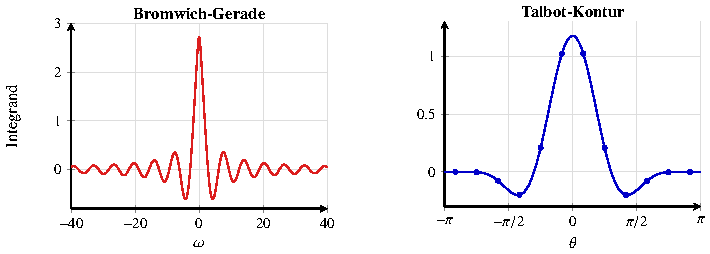
\includegraphics{papers/laplace/images/integrand_vergleich.pdf}
    \caption{Der entlang der Bogenlänge entrollte Realteil des
    Inversionsintegranden für $F(s) = \frac{1}{s}$ bei festem $t$.
    Auf der Bromwich-Geraden (rot) oszilliert die Funktion mit nur
    langsam abfallender Amplitude, auf der Talbot-Kontur (blau) ist sie
    eine glatte, rasch abklingende Kurve, die sich mit wenigen
    Stützstellen präzise integrieren lässt.}
    \label{laplace:fig:integrand_vergleich}
\end{figure}
